\documentclass[11pt,letterpaper,pmlr,twoside]{jmlr}
\usepackage[T1]{fontenc}
\usepackage{lmodern,microtype,mathtools,tikz,booktabs,array}
\usetikzlibrary{arrows.meta,positioning,calc}
\hypersetup{hidelinks,pdftitle={Bounded-Time Logistic SGD Requires Gaussian ReLU Kernel Correlation}}
\hypersetup{pdfauthor={Samuel Mausberg}}
\jmlrproceedings{}{Preprint, October}
\jmlrvolume{}\jmlrpages{}\jmlryear{2026}\jmlrworkshop{}\editor{}
\title[Bounded-time SGD and kernel correlation]{Bounded-Time Logistic SGD Requires\titlebreak Gaussian ReLU Kernel Correlation}
\author[Mausberg]{\Name{Samuel Mausberg}\\\addr Independent Researcher}
\newcommand{\R}{\mathbb R}\newcommand{\E}{\mathbb E}
\newcommand{\X}{\mathcal X}\newcommand{\Hc}{\mathcal H}
\newcommand{\Kc}{\mathcal K}\newcommand{\sgn}{\operatorname{sign}}
\newcommand{\relu}{\operatorname{ReLU}}\newcommand{\dc}{\operatorname{dc}}
\newcommand{\pdc}{\operatorname{pdc}}\newcommand{\sq}{\operatorname{sq}}
\newcommand{\err}{\operatorname{err}}\newcommand{\Risk}{\mathcal E}
\newcommand{\ind}{\mathbf1}\newcommand{\eps}{\varepsilon}
\newcommand{\ip}[2]{\langle #1,#2\rangle}\newcommand{\norm}[1]{\lVert #1\rVert}
\newcommand{\abs}[1]{\lvert #1\rvert}\newcommand{\VC}{\operatorname{VC}}
\newcommand{\op}{\mathrm{op}}\newcommand{\Unif}{\operatorname{Unif}}
\newcommand{\Gcal}{\mathcal G}\newcommand{\Bfr}{\mathfrak B}
\newcommand{\poly}{\operatorname{poly}}
\newcommand{\lean}[1]{\texttt{#1}}
\setlength{\emergencystretch}{1em}
\allowdisplaybreaks[1]
\begin{document}
\maketitle
\begin{abstract}
Feldman, Kamath, and Srebro ask whether a class that Gaussian-initialized logistic SGD on a ReLU network learns under every input distribution must have dimension complexity at most proportional to the number of parameters times the number of steps. We study their two-layer bias-free process on $\{-1,1\}^n$, in which both layers are trained by exact single-example updates and the prediction is the sign of the tail sum of scores. Write $B=\eta mT$ for the effective time. For $B\le12$ and width and step count large relative to $n$ and $B$, we show that the expected error on a target $h$ under a marginal $D$ is at least $1/2-\Delta-9B\,A_D(h)$, where $A_D(h)$ is the label correlation of the Gaussian ReLU features under $D$ and $\Delta$ is an explicit error term. Once width and step count are also large relative to $1/(1/2-\eps)$, learning to error $\eps<1/2$ under every marginal therefore forces correlation at least $(1/2-\eps)/(18B)$ under every marginal. Convex separation turns this into a margin for every target in one fixed kernel, which bounds the VC dimension by $O(B^2)$ and gives an exact deterministic representation of dimension $O(n)$. The margin is very restrictive. Adjacent cube points are within $O(1/\sqrt n)$ of each other in this kernel, so once $n>(18B/(1/2-\eps))^2$ only constant targets can be learned under every marginal; the dimension bound has content only below that threshold. Gates may change during training: at width linear in $n$, a point-mass marginal produces an unbounded number of first-step gate crossings. We also prove a parity lower bound and, in a separate small-step regime, an exact fixed-gate representation with a probabilistic-dimension bound. The proofs of the risk bound, the margin theorem, and the fixed-gate theorem are formalized in Lean 4, apart from the final random-projection step.
\end{abstract}
\begin{keywords}
Stochastic gradient descent; dimension complexity; kernel margin; Gaussian initialization; ReLU networks.
\end{keywords}

\section{Introduction}
\citet{FKS26} ask whether learning under every input distribution by a standard neural training procedure forces a small exact linear representation. Their Open Question~1 fixes the procedure. A fully connected ReLU network with standard Gaussian initialization is trained by single-example logistic SGD, and the prediction is the sign of the sum of the scores over the second half of training. If this procedure learns every target in a class $\Hc$ to expected error $\eps<1/4$ under every input distribution, is the dimension complexity $\dc(\Hc)$ at most $C\cdot ST$, where $S$ is the number of parameters and $T$ the number of steps? We study the two-layer, bias-free case on $\X_n=\{-1,1\}^n$.

Our main result says that, at bounded effective time, the process can beat random guessing on a target and marginal only through the label correlation of one fixed Gaussian ReLU feature map. Let $m$ be the width, $\eta$ the step size, and $B=\eta mT$. For $w\sim N(0,I_n/n)$ let $\Phi(x)=\relu(\ip wx)$, viewed as an element of $\Kc=L^2(N(0,I_n/n))$, and put $A_D(h)=\norm{\E_{x\sim D}h(x)\Phi(x)}_{\Kc}$. Theorem~\ref{thm:risk} shows that if $B\le12$, $m\ge576n$, and $T\ge2B$, then
\begin{equation}
 \Risk(h,D)\ge\frac12-\Delta-9B\,A_D(h)
 \label{eq:intro}
\end{equation}
for every Boolean target $h$ and every marginal $D$, where $\Risk(h,D)$ is the expected error of the process and $\Delta$ is explicit and tends to zero as $m/n$ and $T$ grow at fixed $B$. The bound makes no assumption on the margins of the learned scores.

Under every marginal the bound becomes a representation theorem. Let $\theta=1/2-\eps$. If the process learns $\Hc$ to error $\eps$ under every marginal and $\Delta\le\theta/2$, which holds once $m\ge2^{17}n/\theta$ and $T\ge(216B/\theta)^2$, then $A_D(h)\ge\theta/(18B)$ for all $h\in\Hc$ and all $D$. The vectors $\E_Dh(x)\Phi(x)$ fill the convex hull of $\{h(x)\Phi(x):x\in\X_n\}$, so the point of that hull nearest the origin gives a unit vector $u_h$ with $h(x)\ip{u_h}{\Phi(x)}\ge\theta/(18B)$ at every cube point (Theorem~\ref{thm:margin}). Counting with this margin and applying a random Gaussian projection, as in the classical conversion from margin to dimension \citep{BES02,KMS20}, then give $\dc(\Hc)\le4\cdot10^6(B/\theta)^4(n+1)$. Since $S=m(n+1)$, this confirms Open Question~1 for two-layer networks in this regime, with a deterministic feature map that represents every target exactly. The next two paragraphs explain why the regime is restrictive enough that this confirmation is mainly a statement about what the process cannot learn.

The same margin bounds the VC dimension by $162B^2/\theta^2$, which is $2592B^2$ at $\eps=1/4$ and, since $B\le12$, a constant independent of $n$. The hypothesis of Theorem~\ref{thm:margin} can therefore hold only for classes of bounded VC dimension, and the theorem is best read as a limitation: at bounded effective time the process learns distribution-free only classes that already have a large margin in the Gaussian ReLU kernel. The dimension bound does not follow from the VC bound alone. There are classes on $N$ points with VC dimension $2$ and dimension complexity $\Omega(N^{1/2}/\log N)$ \citep[Theorem~2]{AMY16}, so on the cube a class of bounded VC dimension can have $\dc(\Hc)=2^{\Omega(n)}$; it is the uniform kernel margin that yields dimension linear in $n$.

A two-point marginal makes the limitation sharper. A target that is not constant takes different values at two adjacent points $x$ and $x'$ of the cube. Since ReLU is $1$-Lipschitz, $\norm{\Phi(x)-\Phi(x')}_{\Kc}\le2/\sqrt n$, so the uniform distribution $D$ on $\{x,x'\}$ has $A_D(h)\le1/\sqrt n$, and Theorem~\ref{thm:risk} gives $\Risk(h,D)\ge1/2-\Delta-9B/\sqrt n$ (Corollary~\ref{cor:edge}). Under the hypotheses of Theorem~\ref{thm:margin}, every target in $\Hc$ is therefore constant once $n>(18B/\theta)^2$, which at $\eps=1/4$ and $B=12$ means $n>746{,}496$. Above that dimension the process cannot learn even one nonconstant target under every marginal at bounded effective time, and the dimension bound of Theorem~\ref{thm:margin} matters only for smaller $n$. We keep the dimension bound because it is the representation that the learning premise produces through the kernel margin; the edge argument measures how strong that premise is.

The proof compares the trained network with simpler recurrences. Writing $b=\sqrt m\,a$ makes the initial output coefficients standard Gaussian and gives output-layer steps of size $\gamma=\eta m$ against normalized ReLU features, so $B=\gamma T$ measures the accumulated functional step. The condition on $T$ keeps individual stochastic steps small at fixed $B$. A frozen-feature approximation of the scores usually yields a classification result only after small output margins are controlled. Here that control comes from the initialization. Remove the label-dependent part of the population logistic update, keeping its damping term and the Gaussian output initialization. The resulting recurrence has a symmetric score distribution. At the start of the tail its density is at most $e$ times a Gaussian density, and from there the tail score is strictly increasing along a suitable direction, so a small perturbation of the score changes its sign only with small probability. The labels enter the population update through one vector, their correlation $\mu$ with the normalized initial features. If $\mu$ is small, the trained network stays too close in risk to the symmetric recurrence to beat random guessing by much, and averaging over the hidden layer turns $\norm\mu$ into $A_D(h)$.

Gates need not stay fixed in this regime. At width proportional to $n$, training on a point mass changes an unbounded number of gates at that point in the first step, with probability tending to one (Proposition~\ref{prop:crossings}). The score comparison tolerates these crossings because ReLU is Lipschitz. A different small-step regime, $\eta\le1/m$ with $m\ge16n^2T^2/\delta^2$, keeps every gate at a test point outside an initialization-defined set fixed along every training history. There the tail score is exactly linear in $mn$ gated-coordinate features, which gives the probabilistic-dimension bound of Section~\ref{sec:gate}. That regime allows effective time up to $T$ but yields only an approximate, randomized representation.

The proofs of Theorems~\ref{thm:risk}, \ref{thm:margin}, and~\ref{thm:gate} are formalized in Lean~4 with Mathlib, starting from a definition of the exact process. Section~\ref{sec:lean} describes the formal statements and what remains on paper.

\subsection{Related work}
\paragraph{Kernel-regime analyses.} The relation between small parameter movement and fixed-feature behavior is central to lazy-training theory \citep{Chizat19}, and frozen-gate models that keep products of trained matrices appear in \citet[Section~6.2]{AllenZhu19}. Our score comparison belongs to this line. It uses the Lipschitz property of ReLU across gate boundaries and does not discard the points at which gates change. \citet{JiT20} analyze logistic gradient descent and SGD with gated-coordinate features and Gaussian slab estimates; their output weights are fixed signs and they assume separability in the tangent feature space. \citet{Daniely17} proves conjugate-kernel learning guarantees with resources that depend on a comparator. These works derive learning from a kernel assumption. We argue in the opposite direction: the premise is the classification error that the process achieves, and the kernel margin is the conclusion.

\paragraph{Distribution dependence.} \citet{Malach21} relate gradient-descent learnability under a fixed input distribution to approximation by simpler classes. Their population-gradient theorem assumes a local regularity condition at initialization, and their Remarks~8 and~10 explain that it does not directly cover single-example SGD or ReLU. \citet{Yehudai20} show that gradient methods can fail on a single ReLU neuron under some bounded input distributions, so success under every marginal, the premise here, is a strong requirement. Theorem~\ref{thm:margin} makes precise how strong it is at bounded effective time.

\paragraph{Random features and statistical queries.} \citet{KM25} state an implication from distribution-free gradient descent to random features for a much broader class of models. Their Theorem~3.3 concerns any differentiable model with $p$ parameters and outputs in $[-1,1]$, trained for $T$ steps by mini-batch SGD on the squared loss, with gradients clipped and rounded to a grid of width $c$ and a batch size $b$ satisfying $bc^2\ge\Omega(\log(Tp/\delta))$ for a small constant $\delta>0$. If such a method reaches squared-loss error at most $1/10$ for every source distribution, the theorem asserts that for every prior over targets, most targets can be approximated under every marginal by a linear combination of $\poly(Tp/c^2)$ random features drawn from one law. Even as stated, this conclusion is weaker in kind than Theorem~\ref{thm:margin}. It bounds an average probabilistic dimension, in which the features are random and a fraction of the targets may be approximated poorly or not at all, while Theorem~\ref{thm:margin} gives one deterministic map that represents every target exactly. The precision and batch-size condition also excludes the exact single-example process of Open Question~1. Our result, in turn, covers one architecture at bounded effective time.

The proof of their Theorem~3.3 passes through statistical queries. The rounded mini-batch process is simulated by an SQ algorithm with $Tp$ queries of tolerance $c/8$ \citep[Theorem~3.4, due to \citealt{Abbe21}]{KM25}, which bounds the classical SQ dimension of the class, and then their Theorem~4.1 is invoked, which asserts that the average probabilistic dimension is $O(\sq(\Hc)^{24.01})$. \citet{FKS26} report, citing a personal communication from Karchmer and Malach, that the claimed upper bounds do not hold because of a flaw in the proof. Consistent with that report, \citet{MausbergSQ26} gives an explicit counterexample to Theorem~4.1 under its stated quantifiers: classes of constant classical SQ dimension whose average probabilistic dimension grows without bound. This rules out the intermediate implication on which the proof of Theorem~3.3 relies. It does not disprove the conclusion of Theorem~3.3 about mini-batch SGD. A route that passes only through SQ learnability is closed for a further reason, since distribution-free SQ learnability does not imply small dimension complexity \citep{Patel26,MausbergSQ26}. Our argument works with the dynamics of the process and uses no SQ simulation.

\section{The process and the results}
Let $\X_n=\{-1,1\}^n$, and let $\sgn(z)=1$ for $z\ge0$ and $-1$ otherwise. For a class $\Hc$ of functions $\X_n\to\{-1,1\}$, ordinary dimension complexity is
\begin{equation}
 \dc(\Hc)=\min\left\{d:\exists\phi:\X_n\to\R^d\
 \forall h\in\Hc\ \exists v_h\ \forall x\in\X_n,
 \ h(x)\ip{v_h}{\phi(x)}>0\right\}.
 \label{eq:dc}
\end{equation}
The strict inequality makes the representation exact.

Fix integers $n,m,T\ge1$ and $\eta>0$ before selecting a target $h$ and a marginal $D$. Independently initialize
\begin{equation}
 (W_0)_{ji}\sim N(0,1/n),\qquad (a_0)_j\sim N(0,1/m),
 \qquad f_t(x)=a_t^\top\relu(W_tx).
 \label{eq:init}
\end{equation}
At step $t=0,\ldots,T-1$, draw a fresh $x_t\sim D$, put $y_t=h(x_t)$, and update simultaneously:
\begin{equation}
 \begin{aligned}
 c_t&=\frac{\eta y_t}{1+\exp(y_tf_t(x_t))},
 &v_t&=\ind\{W_tx_t>0\},\\
 a_{t+1}&=a_t+c_t\relu(W_tx_t),
 &W_{t+1}&=W_t+c_t(a_t\odot v_t)x_t^\top.
 \end{aligned}
 \label{eq:actual}
\end{equation}
Both right sides use the old parameters, and a zero preactivation has derivative zero. Put $I_T=\{\lceil T/2\rceil,\ldots,T\}$ and $q=|I_T|$. The returned classifier is $G=\sgn F$, where
\begin{equation}
 F(x)=\frac1q\sum_{t\in I_T}f_t(x).
 \label{eq:tail}
\end{equation}
Dividing by $q$ does not change the sign of the tail sum. The risk is
\[
 \Risk(h,D)=\E_{W_0,a_0,\,(x_t)_{t<T}\sim D^T}
       \Pr_{x\sim D}[G(x)\ne h(x)],
\]
with an independent test point; we write $\err_D(G,h)=\Pr_{x\sim D}[G(x)\ne h(x)]$. The learning premise at error $\eps$ is
\begin{equation}
 \forall h\in\Hc\ \forall D\in\Delta(\X_n),\qquad \Risk(h,D)\le\eps.
 \label{eq:premise}
\end{equation}
The parameters may depend on $\Hc$, $n$, and $\eps$, but they are the same for every pair $(h,D)$.

The proof uses one feature map, fixed before the target and the marginal:
\begin{equation}
 \Phi(x)(w)=\relu(\ip wx),\qquad
 \Kc=L^2\bigl(N(0,I_n/n)\bigr).
 \label{eq:Hilbert}
\end{equation}
For every cube point, $\norm{\Phi(x)}_{\Kc}^2=1/2$. The label correlation of a target under a marginal is
\begin{equation}
 A_D(h)=\left\|\E_{x\sim D}h(x)\Phi(x)\right\|_{\Kc}.
 \label{eq:alignment}
\end{equation}

\begin{theorem}[Risk controlled by kernel correlation]
\label{thm:risk}
Suppose $m\ge576n$, $0<B:=\eta mT\le12$, and $\gamma:=\eta m=B/T\le1/2$. Define
\begin{equation}
 \Delta=\frac{\rho_W}{2}+\rho_a+24\kappa+\frac{27B}{\sqrt T},\qquad
 \rho_W=\min\{1,2^{n+1}e^{-m/16384}\},\quad
 \rho_a=e^{-m/2},\quad \kappa=\frac{544n}{m}.
 \label{eq:Delta}
\end{equation}
For every Boolean target $h$ and every marginal $D$,
\begin{equation}
 \Risk(h,D)\ge\frac12-\Delta-9B A_D(h).
 \label{eq:risk-general}
\end{equation}
\end{theorem}

The bound holds for every Boolean target and every marginal, including point masses. The proof also bounds $\Pr_x[F(x)h(x)<0]$, the error with ties counted as correct that \citet{FKS26} use, so the result does not depend on the convention $\sgn0=1$; it uses the derivative at a zero preactivation only through $\norm{a_t\odot v_t}\le\norm{a_t}$. A concrete instance of the thresholds is the following.

\begin{corollary}[A numerical instance]
\label{cor:instance}
If $m\ge2^{20}n$, $T\ge2^{24}$, and $0<B\le12$, then $\Delta\le471/4096<1/8$, and for every $h$ and $D$,
\begin{equation}
 \Risk(h,D)\ge\frac38-9B A_D(h).
 \label{eq:risk-simple}
\end{equation}
\end{corollary}

Applied to every pair in a learned class, Theorem~\ref{thm:risk} gives the representation theorem.

\begin{theorem}[Kernel margin from success under every marginal]
\label{thm:margin}
Let $0\le\eps<1/2$ and $\theta=1/2-\eps$. Suppose $m\ge576n$, $0<B\le12$, $\gamma\le1/2$, and $\Delta\le\theta/2$. If \eqref{eq:premise} holds for the process \eqref{eq:init}--\eqref{eq:tail}, then $A_D(h)\ge\theta/(18B)$ for every $h\in\Hc$ and every marginal $D$. Consequently each $h\in\Hc$ has a vector $u_h\in\Kc$ with
\begin{equation}
 \norm{u_h}_{\Kc}=1,\qquad
 h(x)\ip{u_h}{\Phi(x)}_{\Kc}\ge\frac{\theta}{18B}
 \quad(x\in\X_n),
 \label{eq:kernelmargin}
\end{equation}
and
\begin{equation}
 \VC(\Hc)\le\frac{162B^2}{\theta^2},
 \qquad
 \dc(\Hc)\le4\cdot10^6\Bigl(\frac B\theta\Bigr)^4(n+1).
 \label{eq:ordinarybound}
\end{equation}
The conditions $m\ge2^{17}n/\theta$ and $T\ge(216B/\theta)^2$ imply $m\ge576n$, $\gamma\le1/2$, and $\Delta\le\theta/2$. The feature map behind the dimension bound is deterministic and may depend on $\Hc$, but not on the target or the marginal.
\end{theorem}

In the regime of Corollary~\ref{cor:instance}, any $\eps<1/4$ gives $\theta>1/4>2\Delta$, so every target has margin at least $1/(72B)$ in $\Kc$ and $\VC(\Hc)\le2592B^2$. Open Question~1 asks for $\dc(\Hc)\le C\cdot ST$ with $S=m(n+1)$ parameters. Theorem~\ref{thm:margin} gives this with a universal constant $C$ for every choice of $m$, $T$, and $\eta$ in that regime, since $B\le12$ and $\theta\ge1/4$ there. The next corollary shows how little the premise allows in high dimension.

\begin{corollary}[Adjacent points]
\label{cor:edge}
Suppose $m\ge576n$, $0<B\le12$, and $\gamma\le1/2$. For every target $h$ that is not constant there is a marginal $D$ supported on two adjacent points of $\X_n$ with
\[
 \Risk(h,D)\ge\frac12-\Delta-\frac{9B}{\sqrt n}.
\]
Consequently, under the hypotheses of Theorem~\ref{thm:margin}, every $h\in\Hc$ is constant if $n>(18B/\theta)^2$.
\end{corollary}

\section{Proof outline}
\label{sec:outline}
Condition first on the initial hidden layer. Its normalized ReLU features are
\[
 \psi(x)=m^{-1/2}\relu(W_0x).
\]
With high probability they satisfy $7/16\le\norm{\psi(x)}^2\le9/16$ at every cube point. On this event and on $\{\norm{a_0}\le2\}$, the tail score of the trained network is within $\kappa$ of a linear logistic-SGD recurrence on the features $\psi$, uniformly over labeled training histories and test points. This estimate allows gates to change. It follows from a bound on the displacement of the input layer and the global Lipschitz property of ReLU.

The linear recurrence has step size $\gamma=\eta m$ and starts at $b_0=\sqrt m\,a_0\sim N(0,I_m)$. Conditionally on each initial vector, its stochastic trajectory differs in mean square by at most $\gamma^2\Lambda T$ from its population recurrence, where $\Lambda=9/16$. Nonexpansivity of logistic gradient steps gives this estimate without an exponential dependence on $T$. Because the estimate holds conditionally, it can later be integrated against the anti-concentration bound, at a classification cost of order $B/\sqrt T$.

Now use the identity
\begin{equation}
 \frac{y}{1+e^{yz}}=\frac y2-\frac12\tanh(z/2)\qquad(y=\pm1).
 \label{eq:logistic-decomp}
\end{equation}
For $\mu=\E_Dh(x)\psi(x)$, the population map is
\[
 v\longmapsto v+\frac\gamma2\mu
      -\frac\gamma2\E_D[\psi(x)\tanh(v^\top\psi(x)/2)].
\]
Deleting $\gamma\mu/2$ gives an odd recurrence that does not depend on the labels. At the start of the tail its density is at most $e$ times the standard Gaussian density, and a directional derivative estimate for the remaining tail gives small-ball probability at most $24r$ on $[-r,r]$. Both steps use bounded effective time: the density bound needs $\lceil T/2\rceil\gamma$ bounded, and the directional estimate needs $B\Lambda/8<1$, that is $B<128/9$. Symmetry makes the risk of this recurrence exactly $1/2$, and restoring the labels moves the tail coefficients by at most $B\norm\mu/2$.

Combining these estimates proves \eqref{eq:risk-general}. The initialization average obeys
\[
 \E_{W_0}\norm{\mu}^2
   =\E_w\left(\E_Dh(x)\relu(\ip wx)\right)^2=A_D(h)^2.
\]
Success under every marginal therefore separates the convex hull of $\{h(x)\Phi(x):x\in\X_n\}$ from the origin. Its nearest point gives \eqref{eq:kernelmargin}. Counting with the margin and a finite Gaussian projection then give ordinary dimension. Figure~\ref{fig:gates} summarizes how gate crossings and signs are handled. The full arguments are in the appendices.

\begin{figure}[htbp]
\centering
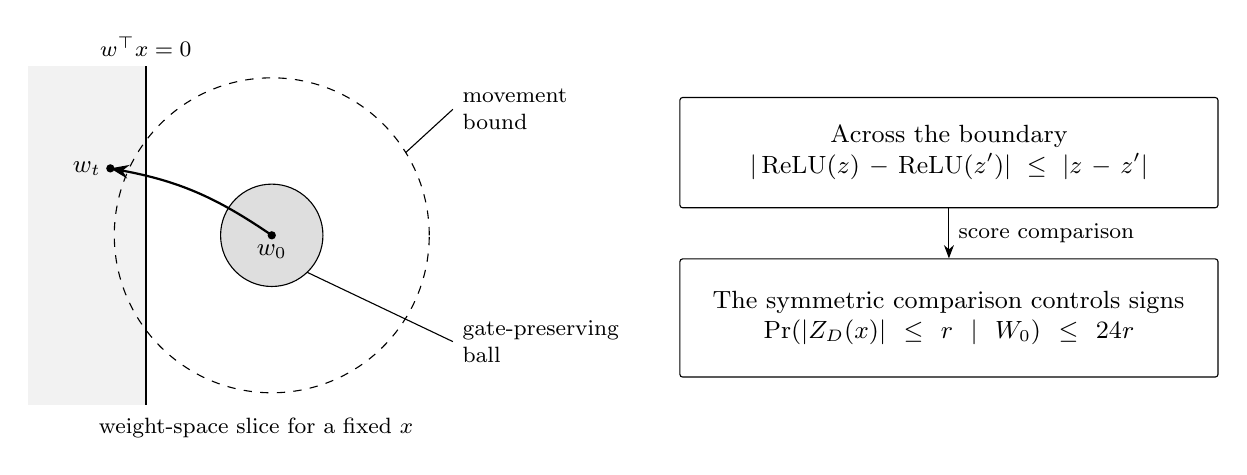
\begin{tikzpicture}[>=Stealth,font=\small]
 \begin{scope}
  \fill[black!5] (-1.5,-2.15) rectangle (0,2.15);
  \draw[thick] (0,-2.15)--(0,2.15);
  \node[above,font=\footnotesize] at (0,2.15) {$w^\top x=0$};
  \fill[black!13] (1.6,0) circle (0.65);
  \draw (1.6,0) circle (0.65);
  \draw[dashed] (1.6,0) circle (2.0);
  \fill (1.6,0) circle (1.5pt);
  \node[below] at (1.6,0) {$w_0$};
  \draw[->,thick] (1.6,0) to[bend right=12] (-0.45,0.85);
  \fill (-0.45,0.85) circle (1.5pt);
  \node[left] at (-0.45,0.85) {$w_t$};
  \draw[thin] (2.05,-0.47)--(3.9,-1.35) node[right,font=\footnotesize,align=left] {gate-preserving\\ball};
  \draw[thin] (3.3,1.05)--(3.9,1.6) node[right,font=\footnotesize,align=left] {movement\\bound};
  \node[below,font=\footnotesize] at (1.4,-2.2) {weight-space slice for a fixed $x$};
 \end{scope}
 \node[draw,rounded corners=1pt,align=center,text width=66mm,minimum height=14mm] (score) at (10.2,1.05)
   {Across the boundary\\$|\relu(z)-\relu(z')|\le|z-z'|$};
 \node[draw,rounded corners=1pt,align=center,text width=66mm,minimum height=15mm] (null) at (10.2,-1.05)
   {The symmetric comparison controls signs\\$\Pr(|Z_D(x)|\le r\mid W_0)\le24r$};
 \draw[->] (score.south)--node[right,font=\footnotesize]{score comparison}(null.north);
\end{tikzpicture}
\caption{Gate stability gives exact frozen-gate identities, and the score bound used here also controls crossings. Signs are controlled through anti-concentration of a label-symmetric comparison score. In the proof, the movement bound is a Frobenius bound on the displacement of the whole input layer.}
\label{fig:gates}
\end{figure}

\section{Gate changes and parity}
The regime allows many activation changes at the test point itself, so an argument that discards every point at which some gate changes would not apply here. The next proposition makes this precise at width proportional to $n$.

\begin{proposition}[First-step crossings at linear width]
\label{prop:crossings}
Fix $C_0\ge2^{20}$, an integer $T_0\ge2^{24}$, and $B\in(0,12]$. For each $n$, set $m_n=\lceil C_0n\rceil$ and $\eta_n=B/(m_nT_0)$. Choose any $x_n\in\X_n$ and train on its point mass with positive label. Let $N_n$ count the rows for which
\[
 w_{0j}^\top x_n>0\quad\text{and}\quad w_{1j}^\top x_n<0.
\]
For every fixed integer $k_0$, $\Pr[N_n\ge k_0]\to1$ as $n\to\infty$. All these schedules satisfy the conditions of Corollary~\ref{cor:instance}.
\end{proposition}

The convergence is slow at these constants. The expected number of candidate rows in the proof is of order $B\sqrt n/(T_0\sqrt{C_0})$, so with $C_0=2^{20}$ and $T_0=2^{24}$ first-step crossings at the test point appear only in very high dimension. The proposition shows that the hypotheses of Theorem~\ref{thm:risk} do not keep the gates fixed, which is what the score comparison needs to handle.

The kernel correlation also yields a direct obstruction for high-order parities. Under the uniform distribution on the cube, the Gaussian law gives every Fourier coefficient of a fixed degree the same expected squared magnitude, and Parseval's identity bounds their sum by $1/2$.

\begin{corollary}[Parity obstruction]
\label{cor:parity}
Under the conditions of Corollary~\ref{cor:instance}, for every $U\subseteq[n]$ with $|U|=k$,
\begin{equation}
 \Risk(\chi_U,\Unif(\X_n))
 \ge\frac38-\frac{9B}{\sqrt{2\binom nk}},
 \qquad \chi_U(x)=\prod_{i\in U}x_i.
 \label{eq:parity}
\end{equation}
In particular, if $\binom nk>2592B^2$, the process does not learn $\chi_U$ to expected error below $1/4$ under the uniform marginal.
\end{corollary}

\section{A fixed-gate regime}
\label{sec:gate}
A different choice of scales keeps the gates fixed. The conclusion is then a probabilistic representation in the sense of \citet{KMS20}, which is weaker than ordinary dimension: by their Theorem~6, a bound on probabilistic dimension alone does not bound ordinary dimension. For $\alpha\ge0$, $\pdc_\alpha(\Hc)$ is the least $d$ for which one law $Q$ of feature maps $\phi:\X_n\to\R^d$ satisfies
\[
 \E_{\phi\sim Q}\inf_{u\in\R^d}\Pr_{x\sim D}\bigl[\sgn\ip u{\phi(x)}\ne h(x)\bigr]\le\alpha
 \qquad\text{for all }h\in\Hc\text{ and }D\in\Delta(\X_n).
\]
The law precedes $h$ and $D$, while $u$ may depend on them and on the realized map. Use the initial gated coordinates
\begin{equation}
 \phi_{W_0}(x)_{j,i}=x_i\ind\{\ip{w_{0j}}x>0\},\qquad 1\le j\le m,\ 1\le i\le n.
 \label{eq:gatefeat}
\end{equation}
For $\tau=\eta T\sqrt n$ and each initialization, define the exceptional set
\begin{equation}
 \Bfr=\bigcup_{j=1}^m\bigl\{x\in\X_n:|\ip{w_{0j}}x|\le\sqrt n\,r_j\bigr\},
 \qquad r_j=|a_{0j}|\sinh\tau+\norm{w_{0j}}(\cosh\tau-1),
 \label{eq:gateset}
\end{equation}
and the bound
\[
 \beta_{n,m}(\tau)=\min\left\{1,\frac{(2/\pi)\sqrt{nm}\sinh\tau+\sqrt{2/\pi}\,m\sqrt{n-1}\,(\cosh\tau-1)}{2-\cosh\tau}\right\}.
\]

\begin{theorem}[Fixed gates at small total step]
\label{thm:gate}
Let $\eta\ge0$ and $\tau=\eta T\sqrt n\le1$.
\begin{enumerate}
\item For every labeled history with labels in $[-1,1]$ and every $x\notin\Bfr$, every gate at $x$ keeps its initial nonzero sign up to time $T$, and $F(x)=\ip{C}{\phi_{W_0}(x)}$ with $C_{ji}=q^{-1}\sum_{t\in I_T}a_{tj}(W_t)_{ji}$.
\item For every fixed marginal $D$, $\E_{W_0,a_0}D(\Bfr)\le \beta_{n,m}(\tau)\le2\sqrt{nm}\,\tau+m\sqrt n\,\tau^2$.
\item If \eqref{eq:premise} holds at error $\eps$, the law of $\phi_{W_0}$ witnesses $\pdc_{\eps+\beta_{n,m}(\tau)}(\Hc)\le mn$. In particular, $\eta\le1/m$ and $m\ge16n^2T^2/\delta^2$ with $0<\delta<1$ give $\pdc_{\eps+\delta}(\Hc)\le mn$.
\end{enumerate}
\end{theorem}

The set $\Bfr$ depends only on the initialization and on $(n,m,T,\eta)$, and part~1 holds for all training histories at once, including histories chosen after seeing the initialization. Only the mass estimate needs the marginal to be fixed in advance. Outside $\Bfr$ the identity in part~1 is exact and keeps every product of trained weights in $C$, so no output margin is needed to transfer classification error. For $0<\eps<1$, taking $\delta=\eps$ gives $\pdc_{2\eps}(\Hc)\le mn<S$, an instance of the probabilistic relaxation proposed by \citet[Section~4]{FKS26}. In this regime $B=\eta mT$ may be as large as $T$, but the width must grow like $n^2T^2$; the two theorems therefore cover different parts of the parameter space, and neither implies the other.

\section{Formal verification}
\label{sec:lean}
We formalized the proofs of Theorems~\ref{thm:risk}, \ref{thm:margin}, and~\ref{thm:gate} in Lean~4 \citep{Lean4} with Mathlib \citep{Mathlib}. The development begins from definitions of the objects in Section~2. The network and the simultaneous update follow \eqref{eq:actual}, with derivative zero at a zero preactivation, and the classifier is the sign of the normalized tail score with $\sgn0=1$. Each hidden row has law $N(0,I_n/n)$ and the output layer has law $N(0,I_m/m)$, both obtained from Mathlib's standard Gaussian measure. A marginal is a probability vector on the cube, so every expectation over training samples or test points is a finite sum, and the risk is the Lebesgue integral over the initialization of the error averaged over histories drawn from $D^T$. For an integrand not known to be measurable, Mathlib's Lebesgue integral is the lower integral. The formal lower bounds on the risk, and the premises that bound it from above, are therefore at least as strong as their counterparts for a measurable integrand, so no measurability hypothesis on the conditional error is needed. The one upper bound on an integral, in part~3 of Theorem~\ref{thm:gate}, comes with a proof that its integrand is measurable. Table~\ref{tab:lean} lists the formal counterparts of the paper's statements. All of them compile without \lean{sorry}, and \lean{\#print axioms} reports only \lean{propext}, \lean{Classical.choice}, and \lean{Quot.sound} for each.

\begin{table}[htbp]
\centering\small
\begin{tabular}{@{}>{\raggedright\arraybackslash}p{0.33\linewidth}>{\raggedright\arraybackslash}p{0.63\linewidth}@{}}
\toprule
Statement & Lean theorems (namespace \lean{GaussianSGD})\\
\midrule
Lemma~\ref{lem:init} & \lean{init\_hidden}, \lean{init\_output}\\
Lemma~\ref{lem:score} & \lean{score\_comparison}, \lean{tail\_score\_comparison}\\
Lemma~\ref{lem:population} & \lean{frozen\_sq\_error}, \lean{label\_effect}, \lean{tail\_sq\_error}, \lean{tail\_label\_effect}\\
Lemma~\ref{lem:density} & \lean{density\_bound}\\
Lemma~\ref{lem:smallball} & \lean{smallball}, \lean{null\_risk}\\
Identity \eqref{eq:kernelidentity} & \lean{kernel\_identity}, \lean{kernelCorr\_eq\_norm}, \lean{Phi\_norm\_sq}\\
Theorem~\ref{thm:risk} & \lean{risk\_lower\_bound}\\
Corollary~\ref{cor:instance} & \lean{lossTerm\_regime}, \lean{risk\_lower\_bound\_regime}\\
Lemma~\ref{lem:geometry}, margin and growth & \lean{margin\_and\_vc}, \lean{growth\_bound}\\
Theorem~\ref{thm:margin}, margin and VC & \lean{kernel\_margin}, \lean{lossTerm\_le\_half}, \lean{regime\_of\_large}\\
Margin $1/(72B)$ for $\eps<1/4$ & \lean{kernel\_margin\_regime}\\
Corollary~\ref{cor:parity} & \lean{parity\_lower\_bound}, \lean{kernelCorr\_parity\_sq\_le}\\
Lemma~\ref{lem:rows} & \lean{row\_movement}\\
Theorem~\ref{thm:gate} & \lean{gates\_fixed}, \lean{exact\_representation}, \lean{gateSet\_mass}, \lean{gateBound\_le}, \lean{measurable\_gate\_inf}, \lean{gate\_pdc}, \lean{gate\_small\_step}\\
\bottomrule
\end{tabular}
\caption{Formal counterparts of the paper's statements. The file \lean{AxiomAudit.lean} prints the axioms of each.}
\label{tab:lean}
\end{table}

Two parts of the paper are not formalized. The first is the dimension bound in Lemma~\ref{lem:geometry} and Theorem~\ref{thm:margin}: the Gaussian projection step, with its chi-square tail bound, is used on paper only, so the formal statements stop at the margin, the VC bound, and the Sauer--Shelah count. The second is Proposition~\ref{prop:crossings}. Several formal proofs take a different route from the text. Nonexpansivity of the logistic maps and the Jacobian estimates \eqref{eq:Jac} and \eqref{eq:derivative} are proved with secant slopes of $\tanh$ and of the logistic function, obtained from the one-variable mean value theorem, without Jacobians of the vector-valued maps. Lemma~\ref{lem:score} bounds the movement of both layers by induction on $t$ in place of the bootstrap over $\bar a$ and $D_W$, and Lemma~\ref{lem:rows} uses the addition formulas for $\cosh$ and $\sinh$ in place of the expansion of the matrix power. The first part of Lemma~\ref{lem:init} evaluates the two Chernoff exponents at $\zeta=\pm1/512$ directly instead of bounding $(\log\mathcal M)''$. The VC bound chooses the signs one at a time with the parallelogram law instead of averaging over random signs. Mathlib does not provide the density of the standard Gaussian measure on $\R^m$, so the formalization identifies it through characteristic functions before applying the change of variables formula in Lemma~\ref{lem:density}.

\section{Scope}
The main theorems hold at bounded effective time. The bound $B\le12$ enters through the density and anti-concentration lemmas, where the method needs $B<128/9$, and it also fixes the constants of the score comparison; we do not know whether success at larger effective time, for instance with $B$ growing with $n$, forces any representation bound. The thresholds on $m$ and $T$ are sufficient conditions chosen to keep the proofs short and do not locate a transition, and the constants are large: at $\eps=1/4$ and $B=12$ the dimension bound is of order $10^{13}(n+1)$. The score comparison allows many gate crossings, but the conclusion is a kernel-regime statement and gives no separation between feature learning and kernel methods. The representation in Theorem~\ref{thm:margin} is existential, since its last step is a random projection, and we give no efficient construction of the feature map.

\section*{AI Disclosure}
Claude (Anthropic) was used to write the Lean~4 formalization described in Section~\ref{sec:lean}, to check the bibliography against publisher and arXiv records, and to revise the exposition. The author is responsible for the results and their presentation.

\begin{thebibliography}{99}
\bibitem[Abbe et~al.(2021)Abbe, Kamath, Malach, Sandon, and Srebro]{Abbe21}
Emmanuel Abbe, Pritish Kamath, Eran Malach, Colin Sandon, and Nathan Srebro.
\newblock On the power of differentiable learning versus {PAC} and {SQ} learning.
\newblock In \emph{Advances in Neural Information Processing Systems}, volume~34, pages 24340--24351, 2021.

\bibitem[Allen-Zhu et~al.(2019)Allen-Zhu, Li, and Liang]{AllenZhu19}
Zeyuan Allen-Zhu, Yuanzhi Li, and Yingyu Liang.
\newblock Learning and generalization in overparameterized neural networks, going beyond two layers.
\newblock In \emph{Advances in Neural Information Processing Systems}, volume~32, 2019.
\newblock arXiv:1811.04918; section numbers refer to version~6.

\bibitem[Alon et~al.(2016)Alon, Moran, and Yehudayoff]{AMY16}
Noga Alon, Shay Moran, and Amir Yehudayoff.
\newblock Sign rank versus {VC} dimension.
\newblock In \emph{Proceedings of the 29th Annual Conference on Learning Theory}, volume~49 of \emph{Proceedings of Machine Learning Research}, pages 47--80, 2016.

\bibitem[Ben-David et~al.(2002)Ben-David, Eiron, and Simon]{BES02}
Shai Ben-David, Nadav Eiron, and Hans~Ulrich Simon.
\newblock Limitations of learning via embeddings in {E}uclidean half spaces.
\newblock \emph{Journal of Machine Learning Research}, 3:441--461, 2002.

\bibitem[Chizat et~al.(2019)Chizat, Oyallon, and Bach]{Chizat19}
L\'ena\"ic Chizat, Edouard Oyallon, and Francis Bach.
\newblock On lazy training in differentiable programming.
\newblock In \emph{Advances in Neural Information Processing Systems}, volume~32, 2019.
\newblock arXiv:1812.07956.

\bibitem[Daniely(2017)]{Daniely17}
Amit Daniely.
\newblock {SGD} learns the conjugate kernel class of the network.
\newblock In \emph{Advances in Neural Information Processing Systems}, volume~30, 2017.
\newblock arXiv:1702.08503.

\bibitem[de~Moura and Ullrich(2021)]{Lean4}
Leonardo de~Moura and Sebastian Ullrich.
\newblock The {L}ean 4 theorem prover and programming language.
\newblock In \emph{Automated Deduction -- CADE 28}, volume 12699 of \emph{Lecture Notes in Computer Science}, pages 625--635. Springer, 2021.

\bibitem[Feldman et~al.(2026)Feldman, Kamath, and Srebro]{FKS26}
Vitaly Feldman, Pritish Kamath, and Nathan Srebro.
\newblock Invited open problem: Is the power of deep learning over linear models inherently distribution dependent?
\newblock In \emph{Proceedings of the 39th Conference on Learning Theory}, volume~336 of \emph{Proceedings of Machine Learning Research}, pages 7117--7122, 2026.

\bibitem[Ji and Telgarsky(2020)]{JiT20}
Ziwei Ji and Matus Telgarsky.
\newblock Polylogarithmic width suffices for gradient descent to achieve arbitrarily small test error with shallow {ReLU} networks.
\newblock In \emph{International Conference on Learning Representations}, 2020.
\newblock arXiv:1909.12292.

\bibitem[Kamath et~al.(2020)Kamath, Montasser, and Srebro]{KMS20}
Pritish Kamath, Omar Montasser, and Nathan Srebro.
\newblock Approximate is good enough: Probabilistic variants of dimensional and margin complexity.
\newblock In \emph{Proceedings of the 33rd Conference on Learning Theory}, volume~125 of \emph{Proceedings of Machine Learning Research}, pages 2236--2262, 2020.

\bibitem[Karchmer and Malach(2025)]{KM25}
Ari Karchmer and Eran Malach.
\newblock The power of random features and the limits of distribution-free gradient descent.
\newblock In \emph{Proceedings of the 42nd International Conference on Machine Learning}, volume 267 of \emph{Proceedings of Machine Learning Research}, pages 29078--29097, 2025.
\newblock Theorem numbers refer to arXiv:2505.10423v1.

\bibitem[Malach et~al.(2021)Malach, Yehudai, Shalev-Shwartz, and Shamir]{Malach21}
Eran Malach, Gilad Yehudai, Shai Shalev-Shwartz, and Ohad Shamir.
\newblock The connection between approximation, depth separation and learnability in neural networks.
\newblock In \emph{Proceedings of the 34th Conference on Learning Theory}, volume~134 of \emph{Proceedings of Machine Learning Research}, pages 3265--3295, 2021.

\bibitem[Mausberg(2026)]{MausbergSQ26}
Samuel Mausberg.
\newblock Distribution-independent {SQ} learning does not imply low dimension complexity.
\newblock Preprint, version 4, October 2026.

\bibitem[{The mathlib Community}(2020)]{Mathlib}
{The mathlib Community}.
\newblock The {L}ean mathematical library.
\newblock In \emph{Proceedings of the 9th ACM SIGPLAN International Conference on Certified Programs and Proofs}, pages 367--381, 2020.

\bibitem[Patel(2026)]{Patel26}
Shyamal Patel.
\newblock A separation between distribution-free {SQ} learning and dimension complexity.
\newblock arXiv:2609.19780v1, 2026.

\bibitem[Yehudai and Shamir(2020)]{Yehudai20}
Gilad Yehudai and Ohad Shamir.
\newblock Learning a single neuron with gradient methods.
\newblock In \emph{Proceedings of the 33rd Conference on Learning Theory}, volume~125 of \emph{Proceedings of Machine Learning Research}, pages 3756--3786, 2020.
\end{thebibliography}

\clearpage
\appendix
\section{Initialization and the score comparison}
\label{app:comparison}
Throughout the appendices recall $\Lambda=9/16$, and let $\lambda=7/16$ and $\psi(x)=m^{-1/2}\relu(W_0x)$. Define the good event
\begin{equation}
 \Gcal=\{W_0:\lambda\le\norm{\psi(x)}^2\le\Lambda\text{ for every }x\in\X_n\}.
 \label{eq:good}
\end{equation}
It is fixed before any target, marginal, or sample history is chosen.

\begin{lemma}[Initialization bounds]
\label{lem:init}
The initialization satisfies
\[
 \Pr(W_0\notin\Gcal)\le\rho_W,
 \qquad \Pr(\norm{a_0}>2)\le\rho_a.
\]
\end{lemma}
\begin{proof}
Fix $x$. The variables $Y_j=\relu(w_{0j}^\top x)^2$ are independent with the law of $Y=Z^2\ind\{Z>0\}$ for $Z\sim N(0,1)$. Its mean is $1/2$ and
\[
 \mathcal M(\zeta)=\E e^{\zeta Y}=\frac{1+(1-2\zeta)^{-1/2}}2.
\]
For $|\zeta|\le1/4$, $\mathcal M\ge1/2$ and $\mathcal M''\le(3/2)2^{5/2}$. Hence $(\log\mathcal M)''\le32$. Since $(\log\mathcal M)'(0)=1/2$, integration gives
\[
 \log\E e^{\zeta(Y-1/2)}\le16\zeta^2.
\]
Apply Chernoff's inequality with $\zeta=\pm1/512$. Each tail at distance $1/16$ from the mean has probability at most $e^{-m/16384}$. A union bound over the $2^n$ points proves the first claim.

Also $m\norm{a_0}^2$ has the $\chi_m^2$ law. Markov's inequality applied to $e^{\chi_m^2/4}$ gives
\[
 \Pr(\norm{a_0}>2)\le e^{-m}2^{m/2}\le e^{-m/2}.
\]
\end{proof}

Put $g(y,z)=y/(1+e^{yz})$. For $y=\pm1$ it has absolute value at most one, and its derivative in $z$ lies between $-1/4$ and zero. On any labeled history, define the linear recurrence
\begin{equation}
 u_0=\sqrt m\,a_0,
 \qquad
 u_{t+1}=u_t+\gamma g(y_t,u_t^\top\psi(x_t))\psi(x_t),
 \qquad \gamma=\eta m,
 \label{eq:frozen}
\end{equation}
driven by the same samples as the network.

\begin{lemma}[Score comparison through gate changes]
\label{lem:score}
Suppose $W_0\in\Gcal$, $\norm{a_0}\le2$, $m\ge576n$, $B\le12$, and $\gamma\le1/2$. For every history with labels $y_t=\pm1$,
\begin{equation}
 \max_{0\le t\le T}\max_{x\in\X_n}
   |f_t(x)-u_t^\top\psi(x)|\le\kappa=544n/m.
 \label{eq:score-compare}
\end{equation}
The same bound holds for the normalized tail scores.
\end{lemma}
\begin{proof}
Write
\[
 \bar a=\max_{t\le T}\norm{a_t},\qquad
 D_W=\max_{t\le T}\norm{W_t-W_0}_F.
\]
From the input-layer updates,
\begin{equation}
 D_W\le\eta T\sqrt n\,\bar a=\frac{B\sqrt n}{m}\bar a.
 \label{eq:DW}
\end{equation}
ReLU is 1-Lipschitz, so
\[
 \norm{\relu(W_tx)}\le\sqrt{m\Lambda}+\sqrt n\,D_W.
\]
Summing the output-layer increments and using \eqref{eq:DW} yields
\[
 \bar a\le\norm{a_0}+B\sqrt{\Lambda/m}+\frac{B^2n}{m^2}\bar a.
\]
Under the hypotheses, $B^2n/m^2\le1/4$ and $B\sqrt{\Lambda/m}\le3/8$. Thus $\bar a<4$ and $D_W\le4B\sqrt n/m$.

Let $b_t=\sqrt m\,a_t$ and define
\[
 e_t(x)=m^{-1/2}\bigl(\relu(W_tx)-\relu(W_0x)\bigr),
 \qquad r_t(x)=f_t(x)-b_t^\top\psi(x).
\]
Uniformly in $t$ and $x$,
\begin{equation}
 \norm{e_t(x)}\le e_*:=\frac{4Bn}{m^{3/2}},
 \qquad |r_t(x)|\le r_*:=\frac{16Bn}{m}.
 \label{eq:residuals}
\end{equation}

For fixed $(x,y)$, the map $\mathcal S_{x,y}(v)=v+\gamma g(y,v^\top\psi(x))\psi(x)$ has derivative $I-\gamma\ell''\psi(x)\psi(x)^\top$, where $\ell''=-\partial_zg(y,z)=e^{yz}/(1+e^{yz})^2\in(0,1/4]$. As $\gamma\le1/2$ and $\norm{\psi(x)}^2\le\Lambda$, this derivative is positive semidefinite with operator norm at most one, so $\mathcal S_{x,y}$ is nonexpansive. Comparing the update of $b_t$ with $\mathcal S_{x_t,y_t}(b_t)$ gives a residual of norm at most
\[
 \gamma\bigl(\sqrt\Lambda\,r_*/4+e_*\bigr).
\]
Iterating nonexpansivity from $b_0=u_0$ proves
\[
 \norm{b_t-u_t}\le B\bigl(\sqrt\Lambda\,r_*/4+e_*\bigr).
\]
Consequently,
\[
 |f_t(x)-u_t^\top\psi(x)|
 \le(1+B\Lambda/4)r_*+B\sqrt\Lambda\,e_*.
\]
The first term is at most $516n/m$. The second is at most $432n/m^{3/2}\le18n/m$, since $m\ge576$. Their sum is at most $534n/m\le544n/m$. Averaging over $I_T$ preserves the bound.
\end{proof}

\section{Population comparison and Gaussian anti-concentration}
\label{app:null}
Fix $W_0\in\Gcal$, a Boolean target $h$, and a marginal $D$. Let
\[
 \mu=\E_D h(x)\psi(x),\qquad
 R(v)=v-\frac\gamma2\E_D\left[\psi(x)\tanh\bigl(v^\top\psi(x)/2\bigr)\right].
\]
The map $R$ is odd. Its derivative is
\begin{equation}
 DR(v)=I-\gamma H(v),\qquad
 H(v)=\frac14\E_D\left[\psi(x)\psi(x)^\top
             \operatorname{sech}^2\bigl(v^\top\psi(x)/2\bigr)\right],
 \label{eq:H}
\end{equation}
and $0\preceq H(v)\preceq(\Lambda/4)I$. Both $R$ and $R+\gamma\mu/2$ are nonexpansive when $\gamma\le1/2$.

With the same initial vector $b_0=\sqrt m\,a_0$, define the population and symmetric recurrences
\begin{equation}
 v_0=z_0=b_0,
 \qquad v_{t+1}=R(v_t)+\gamma\mu/2,
 \qquad z_{t+1}=R(z_t).
 \label{eq:population}
\end{equation}
By \eqref{eq:logistic-decomp}, $v\mapsto R(v)+\gamma\mu/2$ is the conditional mean of one step of \eqref{eq:frozen}.

\begin{lemma}[Sampling and label effects]
\label{lem:population}
Assume $W_0\in\Gcal$ and $\gamma\le1/2$. Conditionally on $W_0$ and $b_0$, for $t\le T$,
\begin{equation}
 \E\norm{u_t-v_t}^2\le t\gamma^2\Lambda.
 \label{eq:samplevariance}
\end{equation}
For every $b_0$,
\begin{equation}
 \norm{v_t-z_t}\le t\gamma\norm\mu/2.
 \label{eq:labeldifference}
\end{equation}
In particular, if $\bar u=q^{-1}\sum_{t\in I_T}u_t$ and similarly for $\bar v$ and $\bar z$, then
\begin{equation}
 \E\bigl[\norm{\bar u-\bar v}^2\bigm| W_0,b_0\bigr]
 \le\frac{\Lambda B^2}{T},
 \qquad
 |\ip{\bar v-\bar z}{\psi(x)}|\le\frac{3B}{8}\norm\mu\quad(x\in\X_n).
 \label{eq:tailcomparisons}
\end{equation}
\end{lemma}
\begin{proof}
Let $P=R+\gamma\mu/2$. Given the past, the sample update \eqref{eq:frozen} has conditional mean $P(u_t)$. Write it as $P(u_t)+\gamma\xi_t$, where $\E[\xi_t\mid\text{past}]=0$ and
\[
 \E[\norm{\xi_t}^2\mid\text{past}]
 \le\E_D\norm{g(h(x),u_t^\top\psi(x))\psi(x)}^2\le\Lambda.
\]
The cross term vanishes in the conditional second moment, so nonexpansivity of $P$ gives
\[
 \E[\norm{u_{t+1}-v_{t+1}}^2\mid\text{past}]
 \le\norm{u_t-v_t}^2+\gamma^2\Lambda.
\]
Induction proves \eqref{eq:samplevariance}. Nonexpansivity of $R$ gives
$\norm{v_{t+1}-z_{t+1}}\le\norm{v_t-z_t}+\gamma\norm\mu/2$, which proves \eqref{eq:labeldifference}. Jensen's inequality for the tail average and $t\gamma^2\Lambda\le T\gamma^2\Lambda=\Lambda B^2/T$ give the first assertion of \eqref{eq:tailcomparisons}. The second uses $\norm{\psi(x)}\le\sqrt\Lambda=3/4$ and $t\gamma\le B$.
\end{proof}

\begin{lemma}[Density at the beginning of the tail]
\label{lem:density}
Assume $\norm{\psi(x)}^2\le\Lambda$ for all $x$, $B\le12$, and $\gamma\le1/2$, and put $s=\lceil T/2\rceil$. For $b_0\sim N(0,I_m)$ and every Borel set $E\subseteq\R^m$,
\begin{equation}
 \Pr(z_s\in E)\le e\,\Pr(b_0\in E).
 \label{eq:density}
\end{equation}
Equivalently, $z_s$ has a density bounded by $e\,(2\pi)^{-m/2}\exp(-\norm v^2/2)$.
\end{lemma}
\begin{proof}
For every $v$, the matrix $H(v)$ is positive semidefinite with $\operatorname{tr}H(v)\le\Lambda/4$, since $\operatorname{sech}^2\le1$ and $\E_D\norm{\psi(x)}^2\le\Lambda$. Let $\omega=\gamma\Lambda/4\le9/128$. The eigenvalues $\nu_1,\ldots,\nu_m$ of $\gamma H(v)$ are nonnegative with $\sum_i\nu_i\le\omega$, so
\[
 \det DR(v)=\prod_{i=1}^m(1-\nu_i)\ge1-\sum_{i=1}^m\nu_i\ge1-\omega.
\]
The trace bound keeps this factor independent of the width. Since $\tanh$ is increasing and $1$-Lipschitz, $\ip{R(v)-R(v')}{v-v'}\ge(1-\omega)\norm{v-v'}^2$, so $R$ is injective. Also $R$ is nonexpansive and fixes zero, so $\norm{R(b)}\le\norm b$ and $\varphi(R(b))\ge\varphi(b)$ for the standard Gaussian density $\varphi$.

Fix a Borel set $E$ and put $E'=R^{-1}(E)$, so that $R(E')\subseteq E$. The change of variables formula for the injective map $R$ gives
\[
 \Pr(b_0\in E)\ge\int_{R(E')}\varphi
 =\int_{E'}\det DR(b)\,\varphi(R(b))\,db
 \ge(1-\omega)\Pr(b_0\in E').
\]
Thus the law of $R(b_0)$ is at most $(1-\omega)^{-1}$ times the standard Gaussian law. Pushing forward by $R$ preserves such a domination, so by induction the law of $z_s=R^s(b_0)$ is at most $(1-\omega)^{-s}$ times the standard Gaussian law. Finally $(1-\omega)^{-s}\le\exp(s\omega/(1-\omega))\le e$, because $s\omega\le1-\omega$: indeed $\gamma(s+1)\le(B+\gamma)/2+\gamma\le27/4$, so $\omega(s+1)=9\gamma(s+1)/64\le243/256$. This proves \eqref{eq:density}.
\end{proof}

\begin{lemma}[Anti-concentration of the symmetric tail]
\label{lem:smallball}
Assume $W_0\in\Gcal$, $B\le12$, and $\gamma\le1/2$. For each $x\in\X_n$, let
\[
 Z_D(x;b_0)=\ip{\bar z(b_0)}{\psi(x)},\qquad b_0\sim N(0,I_m).
\]
For every $r\ge0$,
\begin{equation}
 \Pr_{b_0}(|Z_D(x;b_0)|\le r\mid W_0)\le24r.
 \label{eq:smallball}
\end{equation}
The law of $Z_D(x;b_0)$ is symmetric and has no atom at zero. Hence, for every Boolean $h$,
\begin{equation}
 \E_{b_0}\err_D(\sgn Z_D(\cdot;b_0),h)=1/2.
 \label{eq:nullrisk}
\end{equation}
\end{lemma}
\begin{proof}
Put $s=\lceil T/2\rceil$ and $L=T-s$, and regard the tail as a function of $v=z_s$. Write $z^{[v]}_0=v$ and $z^{[v]}_{j+1}=R(z^{[v]}_j)$ for $0\le j<L$. The Jacobians $J_j=D_vz^{[v]}_j$ obey
\[
 J_0=I,\qquad J_{j+1}=(I-\gamma H(z^{[v]}_j))J_j.
\]
Each factor is a contraction, so $\norm{J_j}_{\op}\le1$. Summing
$J_{j+1}-J_j=-\gamma H(z^{[v]}_j)J_j$ gives
\begin{equation}
 \norm{J_j-I}_{\op}\le j\gamma\Lambda/4
       \le B\Lambda/8\le27/32.
 \label{eq:Jac}
\end{equation}
Since $e^\top Je\ge1-\norm{J-I}_{\op}$ for every unit vector $e$, this bound suffices below, although the $J_j$ need not be symmetric.

Suppose first that $v$ is standard Gaussian. For fixed $x$, put $e_x=\psi(x)/\norm{\psi(x)}$ and decompose $v=\beta e_x+v_\perp$. Conditionally on $v_\perp$, $\beta$ is a standard Gaussian. At every $\beta$ and $v_\perp$,
\begin{align}
 \frac{d}{d\beta}\left[\frac1{L+1}\sum_{j=0}^L
             \ip{z^{[v]}_j}{\psi(x)}\right]
 &=\norm{\psi(x)}\,e_x^\top
     \left(\frac1{L+1}\sum_{j=0}^L J_j\right)e_x\notag\\
 &\ge\sqrt\lambda\,(1-B\Lambda/8)
 \ge\frac{5\sqrt7}{128}.
 \label{eq:derivative}
\end{align}
The preimage of $[-r,r]$ in $\beta$ is therefore an interval of length at most $256r/(5\sqrt7)$, and the maximum of the one-dimensional Gaussian density bounds its probability by
\[
 \frac{256r}{5\sqrt{14\pi}}<8r.
\]
By Lemma~\ref{lem:density} the law of the actual $z_s$ is at most $e$ times the standard Gaussian law, so the actual small-ball probability is at most $8er<24r$.

The recurrence $R$ is odd, so $Z_D(x;-b_0)=-Z_D(x;b_0)$. The small-ball estimate excludes an atom at zero. Symmetry then gives error $1/2$ at every fixed test point, and averaging over $D$ proves \eqref{eq:nullrisk}.
\end{proof}

\section{Proofs of the main theorems}
\label{app:margin}
\begin{proof}[Proof of Theorem~\ref{thm:risk}]
Fix $h$ and $D$ before initialization, and condition on $W_0\in\Gcal$. For a test point $x$, put
\[
 Z=Z_D(x;b_0),\qquad
 d_0=\kappa+\frac{3B}{8}\norm\mu,\qquad
 E_x=\ip{\bar u-\bar v}{\psi(x)}.
\]
Lemmas~\ref{lem:score} and~\ref{lem:population} show that on $\{\norm{a_0}\le2\}$,
\[
 |F(x)-Z|\le d_0+|E_x|,\qquad
 \E[|E_x|^2\mid W_0,b_0]\le\sigma^2:=\frac{\Lambda^2 B^2}{T}.
\]
The second bound holds conditionally on every $b_0$. This lets us integrate the error probability against the Gaussian initialization with no independence between $E_x$ and $Z$.

If $\sgn F(x)\ne\sgn Z$, then $|Z|\le|F(x)-Z|$. Conditionally on $b_0$ with $\norm{a_0}\le2$ and $|Z|>d_0$, Markov's inequality therefore bounds the probability of disagreement by $\min\{1,\sigma^2/(|Z|-d_0)^2\}$. Give this minimum the value one when $|Z|\le d_0$. By the layer-cake formula and Lemma~\ref{lem:smallball}, its expectation over the initialization is at most
\begin{align*}
 \int_0^1\Pr_{b_0}\left(|Z|\le d_0+\frac{\sigma}{\sqrt t}\,\middle|\,W_0\right)dt
 &\le24\int_0^1\left(d_0+\frac{\sigma}{\sqrt t}\right)dt\\
 &=24d_0+48\sigma.
\end{align*}
The symmetric classifier has expected error $1/2$. Averaging over the test marginal and adding the probability of $\{\norm{a_0}>2\}$ to the disagreement gives
\[
 \E[\err_D(G,h)\mid W_0]
 \ge\frac12-\rho_a-24\kappa-\frac{27B}{\sqrt T}-9B\norm\mu.
\]
The event $\{\norm{a_0}>2\}$ is paid for separately because Lemma~\ref{lem:smallball} uses the unconditioned Gaussian law of $b_0$.

For initializations outside $\Gcal$, keep only the nonnegativity of the risk. After averaging,
\[
 \Risk(h,D)\ge\frac12(1-\rho_W)-\rho_a-24\kappa-\frac{27B}{\sqrt T}
       -9B\E[\ind_{\Gcal}\norm\mu].
\]
The hidden rows are independent and identically distributed, which gives the exact identity
\begin{align}
 \E_{W_0}\norm\mu^2
 &=\frac1m\sum_{j=1}^m\E_{w_{0j}}
       \left(\E_Dh(x)\relu(w_{0j}^\top x)\right)^2\notag\\
 &=A_D(h)^2.
 \label{eq:kernelidentity}
\end{align}
Thus $\E[\ind_{\Gcal}\norm\mu]\le A_D(h)$ by the Cauchy--Schwarz inequality. This proves \eqref{eq:risk-general}.
\end{proof}

\begin{proof}[Proof of Corollary~\ref{cor:instance}]
The conditions give $m\ge576n$ and $\gamma=B/T\le12/2^{24}<1/2$, so Theorem~\ref{thm:risk} applies. Also $\rho_W,\rho_a\le1/64$ and
\[
 \frac{27B}{\sqrt T}\le\frac{324}{4096},\qquad
 24\kappa\le\frac{51}{4096}.
\]
With $\rho_W/2\le32/4096$ and $\rho_a\le64/4096$, the total loss is at most $471/4096<1/8$, and \eqref{eq:risk-general} gives \eqref{eq:risk-simple}.
\end{proof}

\begin{lemma}[Convex separation and ordinary dimension]
\label{lem:geometry}
Let $X$ be a nonempty finite set with $M$ points, let $\Phi:X\to\Kc$ satisfy $\norm{\Phi(x)}^2\le1/2$, and let $c>0$. Suppose a nonempty class $\Hc$ of functions $X\to\{-1,1\}$ satisfies
\begin{equation}
 \norm{\E_{x\sim D}h(x)\Phi(x)}\ge c\qquad\text{for all }h\in\Hc\text{ and }D\in\Delta(X).
 \label{eq:allmarginal}
\end{equation}
Then every $h\in\Hc$ has a unit vector $u_h$ with $h(x)\ip{u_h}{\Phi(x)}\ge c$ for all $x$, and $\VC(\Hc)\le1/(2c^2)$. With $v=\lfloor1/(2c^2)\rfloor$,
\[
 |\Hc|\le\sum_{i=0}^{v}\binom Mi\le(M+1)^v,\qquad
 \dc(\Hc)\le1+\frac{32(v+2)}{c^2}\log(M+1).
\]
\end{lemma}
\begin{proof}
For fixed $h$, the convex hull
\[
 C_h=\operatorname{conv}\{h(x)\Phi(x):x\in X\}
\]
is compact in a finite-dimensional subspace, and its elements are exactly the vectors $\E_Dh(x)\Phi(x)$, one for each marginal $D$. This is where the hypothesis over all marginals enters: if $p_h$ is the point of $C_h$ nearest to zero, then $\norm{p_h}\ge c$. Minimizing the squared norm along the segment from $p_h$ to any $z\in C_h$ gives
\[
 \ip{p_h}{z-p_h}\ge0.
\]
Thus $u_h=p_h/\norm{p_h}$ has the stated margin at every point. It depends on $h$ but not on $D$.

Suppose $r$ points are shattered. For every sign vector $s\in\{-1,1\}^r$, the unit vector of a target realizing $s$ gives
\[
 rc\le\left\|\sum_{i=1}^rs_i\Phi(x_i)\right\|.
\]
Averaging the square over independent fair signs gives $r^2c^2\le r/2$, so $r\le1/(2c^2)$. The Sauer--Shelah lemma then gives the bound on $|\Hc|$.

It remains to project the finite collection of input and target vectors. All of them lie in the span of $\Phi(X)$, which is finite-dimensional. A matrix $J$ with independent $N(0,1/d)$ entries satisfies, for each fixed vector $z$ and $0<\xi\le1/2$,
\[
 \Pr\left(\big|\norm{Jz}^2-\norm z^2\big|>\xi\norm z^2\right)
 \le2e^{-d\xi^2/8},
\]
by the elementary chi-square Chernoff bound. Apply it to $u_h+\Phi(x)$ and $u_h-\Phi(x)$ for all $h$ and $x$, with $\xi=c/2\le2^{-3/2}$. Since $4|\Hc|Me^{-dc^2/32}<1$ for some integer $d\le1+32c^{-2}\log(4|\Hc|M)$, some realization of $J$ preserves all these squared norms to relative error $\xi$. Polarization then bounds each inner-product error by
\[
 \frac\xi2\bigl(\norm{u_h}^2+\norm{\Phi(x)}^2\bigr)
 \le\frac{3c}{8}<c,
\]
so $J\Phi(x)$ and $Ju_h$ represent every target exactly. Finally $\log(4|\Hc|M)\le\log(4M)+v\log(M+1)\le(v+2)\log(M+1)$.
\end{proof}

\begin{proof}[Proof of Theorem~\ref{thm:margin}]
Fix $h\in\Hc$ and $D$. By Theorem~\ref{thm:risk} and \eqref{eq:premise}, $1/2-\Delta-9BA_D(h)\le\eps$, so $9BA_D(h)\ge\theta-\Delta\ge\theta/2$. Hence \eqref{eq:allmarginal} holds with $c=\theta/(18B)$, and Lemma~\ref{lem:geometry} with $M=2^n$ gives \eqref{eq:kernelmargin} and $\VC(\Hc)\le1/(2c^2)=162B^2/\theta^2$. For the dimension bound put $K=c^{-2}=324B^2/\theta^2$. If $\Hc$ is empty there is nothing to prove. Otherwise $c\le\norm{\Phi(x)}=2^{-1/2}$, so $K\ge2$ and $v+2\le K/2+2\le3K/2$. With $\log(2^n+1)\le(n+1)\log2$, the lemma gives
\[
 \dc(\Hc)\le1+48\log2\cdot K^2(n+1)\le34K^2(n+1)\le4\cdot10^6\Bigl(\frac B\theta\Bigr)^4(n+1).
\]

For the sufficient conditions, suppose $m\ge2^{17}n/\theta$ and $T\ge(216B/\theta)^2$. Since $\theta\le1/2$, $m\ge2^{18}n\ge576n$. If $2B\le1$ then $T\ge1\ge2B$; otherwise $T\ge(432B)^2\ge2B$. So $\gamma=B/T\le1/2$. Next, $24\kappa=13056n/m\le13056\,\theta/2^{17}<\theta/8$. Put $y=8/\theta\ge16$. Then $m/16384\ge ny$, so $\rho_W/2\le2^ne^{-ny}=e^{-n(y-\log2)}\le e^{-(y-\log2)}\le1/y=\theta/8$, since $n\ge1$ and $y-\log2\ge\log y$ for $y\ge16$. Also $\rho_a=e^{-m/2}\le e^{-y}<\theta/8$, and $27B/\sqrt T\le\theta/8$. Summing, $\Delta\le\theta/2$.
\end{proof}

\begin{proof}[Proof of Corollary~\ref{cor:edge}]
The cube graph, with edges between points that differ in one coordinate, is connected. If $h$ is not constant, some edge $\{x,x'\}$ therefore has $h(x')=-h(x)$; let $i$ be the coordinate in which $x$ and $x'$ differ, and let $D$ be the uniform distribution on $\{x,x'\}$. Then $\E_Dh\Phi=\tfrac12h(x)(\Phi(x)-\Phi(x'))$. Since ReLU is $1$-Lipschitz and $w\sim N(0,I_n/n)$,
\[
 \norm{\Phi(x)-\Phi(x')}_{\Kc}^2\le\E_w\ip w{x-x'}^2=4\E_ww_i^2=\frac4n,
\]
so $A_D(h)\le1/\sqrt n$, and Theorem~\ref{thm:risk} gives the first claim. Under the hypotheses of Theorem~\ref{thm:margin}, a nonconstant $h\in\Hc$ would satisfy $\eps\ge\Risk(h,D)\ge1/2-\theta/2-9B/\sqrt n$, that is $\sqrt n\le18B/\theta$.
\end{proof}

\section{Proofs of the crossing and parity statements}
\label{app:consequences}
\begin{proof}[Proof of Proposition~\ref{prop:crossings}]
Write $z_j=w_{0j}^\top x_n$ and $b_j=\sqrt m\,a_{0j}$. The pairs $(z_j,b_j)$ are independent pairs of independent standard Gaussians. The initial score
\[
 f_0(x_n)=m^{-1/2}\sum_j b_j\relu(z_j)
\]
has mean zero and variance $1/2$ for every $n$ and $m$.

Fix $r_0>0$. On $\{f_0(x_n)\le r_0\}$, an initially active row updates according to
\[
 w_{1j}^\top x_n=z_j+\frac{\eta_n n\,b_j}{\sqrt m(1+e^{f_0(x_n)})},
\]
where the update uses the old output coefficient, as simultaneous SGD requires. The row becomes strictly negative whenever
\[
 b_j\le-1,\qquad 0<z_j<d_n,
 \qquad d_n=\frac{\eta_n n}{\sqrt m(1+e^{r_0})}.
\]
Let $C_n$ count these candidate rows. It is binomial, and
\[
 \E C_n=m\Pr(b_j\le-1)\Pr(0<z_j<d_n)
 \asymp_{r_0}\frac{B n}{T_0\sqrt m}\longrightarrow\infty,
\]
because $m=\lceil C_0n\rceil$, $d_n\to0$, and $B$, $C_0$, $T_0$, $r_0$ are fixed. Therefore $\Pr(C_n<k_0)\to0$ for every fixed $k_0$. The count $C_n$ and the initial score are dependent, but the union bound and the variance of the score give
\[
 \Pr(N_n<k_0)\le\Pr(C_n<k_0)+\Pr(f_0(x_n)>r_0)
 \le\Pr(C_n<k_0)+\frac1{2r_0^2}.
\]
Take the upper limit in $n$, then let $r_0\to\infty$.
\end{proof}

\begin{proof}[Proof of Corollary~\ref{cor:parity}]
For each $w$, let $\widehat r_w(U)=\E_{x\sim\Unif(\X_n)}\chi_U(x)\relu(w^\top x)$. The Gaussian law is invariant under coordinate permutations, so
\[
 \ell_k=\E_w\widehat r_w(U)^2
\]
depends only on $|U|=k$. Parseval's identity and nonnegativity give
\[
 \binom nk\ell_k
 \le\sum_{U\subseteq[n]}\E_w\widehat r_w(U)^2
 =\E_w\E_x\relu(w^\top x)^2=\frac12.
\]
Since $A_{\Unif}(\chi_U)^2=\ell_k$, substituting in \eqref{eq:risk-simple} proves \eqref{eq:parity}. The right side exceeds $1/4$ whenever $\binom nk>2592B^2$.
\end{proof}

\section{Proofs for the fixed-gate regime}
\label{app:gate}
Write $\nu=\eta\sqrt n$. The labels may be any numbers in $[-1,1]$, so $|c_t|\le\eta$.

\begin{lemma}[Row movement]
\label{lem:rows}
For every initialization, every labeled history, and every row $j$,
\[
 |a_{tj}|\le|a_{0j}|\cosh(t\nu)+\norm{w_{0j}}\sinh(t\nu),\qquad
 \norm{w_{tj}-w_{0j}}\le|a_{0j}|\sinh(t\nu)+\norm{w_{0j}}\bigl(\cosh(t\nu)-1\bigr).
\]
No restriction on $\eta$ is needed.
\end{lemma}
\begin{proof}
Fix a row and write $\mathfrak a_t=|a_{tj}|$ and $\mathfrak w_t=\norm{w_{tj}}$. Since $|c_t|\le\eta$ and $\norm{x_t}=\sqrt n$, the updates give $\mathfrak a_{t+1}\le \mathfrak a_t+\nu \mathfrak w_t$ and $\mathfrak w_{t+1}\le \mathfrak w_t+\nu \mathfrak a_t$. The $t$-th power of $\begin{psmallmatrix}1&\nu\\\nu&1\end{psmallmatrix}$ has diagonal entries $E_t=\sum_{r\text{ even}}\binom tr\nu^r$ and off-diagonal entries $O_t=\sum_{r\text{ odd}}\binom tr\nu^r$, and $\binom tr\le t^r/r!$ gives $E_t\le\cosh(t\nu)$ and $O_t\le\sinh(t\nu)$. This proves the first bound. For the displacement, sum the increments: $\norm{w_{tj}-w_{0j}}\le\nu\sum_{r<t}\mathfrak a_r\le O_tu_0+(E_t-1)\mathfrak w_0$, using $O_{t+1}=O_t+\nu E_t$ and $E_{t+1}=E_t+\nu O_t$.
\end{proof}

\begin{proof}[Proof of Theorem~\ref{thm:gate}]
Put $\sigma_\tau=\sinh\tau$ and $\omega_\tau=\cosh\tau-1$. If $x\notin\Bfr$, the Cauchy--Schwarz inequality and Lemma~\ref{lem:rows} give, for every row and every $t\le T$,
\[
 |\ip{w_{tj}-w_{0j}}x|\le\sqrt n\,r_j<|\ip{w_{0j}}x|,
\]
so every preactivation at $x$ keeps its initial nonzero sign along every history. On such a point, $f_t(x)=\sum_ja_{tj}\ind\{\ip{w_{0j}}x>0\}\ip{w_{tj}}x=\sum_{j,i}a_{tj}(W_t)_{ji}\,\phi_{W_0}(x)_{j,i}$, and averaging over $I_T$ proves part~1.

For part~2 fix $x$ and a row $j$, and write $w_{0j}=Z/\sqrt n$ with $Z\sim N(0,I_n)$. Then $\Gamma=\ip{w_{0j}}x\sim N(0,1)$ and $\norm Z^2=\Gamma^2+V^2$, where $V$ is independent of $\Gamma$ with $\E V\le\sqrt{n-1}$; both are independent of $a_{0j}$. The radius $r_j$ depends on $\norm{w_{0j}}$, and hence on $\Gamma$. The $j$-th event in \eqref{eq:gateset} implies
\[
 |\Gamma|\le\sqrt n\,|a_{0j}|\sigma_\tau+\omega_\tau\sqrt{\Gamma^2+V^2}\le\sqrt n\,|a_{0j}|\sigma_\tau+\omega_\tau|\Gamma|+\omega_\tau V,
\]
and since $\omega_\tau<1$ for $\tau\le1$, it is contained in $\{|\Gamma|\le(\sqrt n|a_{0j}|\sigma_\tau+\omega_\tau V)/(1-\omega_\tau)\}$, whose right side is independent of $\Gamma$. The standard Gaussian density is at most $1/\sqrt{2\pi}$ and $\E|a_{0j}|=\sqrt{2/(\pi m)}$, so this event has probability at most
\[
 \frac{(2/\pi)\sqrt{n/m}\,\sigma_\tau+\sqrt{2/\pi}\sqrt{n-1}\,\omega_\tau}{1-\omega_\tau}.
\]
A union bound over the rows gives $\Pr(x\in\Bfr)\le \beta_{n,m}(\tau)$ for each fixed $x$, and averaging over a fixed marginal gives $\E D(\Bfr)\le \beta_{n,m}(\tau)$. The estimate is for a fixed $x$, which is why part~2 needs the marginal to be fixed in advance. For the simpler bound, $0\le\tau\le1$ gives $\sinh\tau\le6\tau/5$, $\cosh\tau-1\le5\tau^2/9$, and $2-\cosh\tau\ge4/9$; with $2/\pi<2/3$ and $\sqrt{2/\pi}<4/5$ this yields $\beta_{n,m}(\tau)\le2\sqrt{nm}\,\tau+m\sqrt n\,\tau^2$.

For part~3 fix $h$ and $D$. Pathwise, part~1 gives $\err_D(\sgn\ip C{\phi_{W_0}},h)\le\err_D(G,h)+D(\Bfr)$. The infimum over $u$ of $\err_D(\sgn\ip u{\phi_{W_0}},h)$ depends only on $W_0$ and is at most the error of every array $C$, whatever $a_0$ and the samples. Averaging gives
\[
 \E_{W_0}\inf_u\err_D(\sgn\ip u{\phi_{W_0}},h)\le\Risk(h,D)+\E D(\Bfr)\le\eps+\beta_{n,m}(\tau).
\]
Finally, if $\eta\le1/m$ and $m\ge16n^2T^2/\delta^2$, then $\tau\le T\sqrt n/m\le\delta^2/(16n^{3/2}T)<1$ and $\beta_{n,m}(\tau)\le2nT/\sqrt m+n^{3/2}T^2/m\le\delta/2+\delta^2/(16\sqrt n)<\delta$.
\end{proof}

\end{document}
